\documentclass{sig-alternate-10pt}
%\documentclass[10pt, conference, letterpaper]{IEEEtran}
\newcommand{\ie}{{\em i.e.}}
\newcommand{\eg}{{\em e.g.}}
\long\def\comment#1{}
\long\def\comment#1{}
\usepackage[utf8]{inputenc}
\usepackage{cleveref}
\crefname{section}{§}{§§}
\Crefname{section}{§}{§§}

% Load basic packages
\usepackage[table,xcdraw]{xcolor}
\usepackage{balance}  % to better equalize the last page
\usepackage{graphicx}
\usepackage{subfigure}
\usepackage{graphics} % for EPS, load graphicx instead
\usepackage{times}    % comment if you want LaTeX's default font
\usepackage[hyphens]{url}      % llt: nicely formatted URLs
\usepackage{array}
\usepackage{enumerate}
\usepackage{amsmath}
\usepackage{textcomp}
\usepackage{flushend}
\usepackage[utf8]{inputenc}
\usepackage{amsmath}
\usepackage{dirtytalk}
\usepackage{csquotes}
\usepackage{xspace}
\newcommand*\textfrac[2]{
  \frac{\text{#1}}{\text{#2}}
}
\usepackage{algorithm}
\usepackage{xspace}
%\usepackage{algorithmicx}
\usepackage[noend]{algpseudocode}

\newcommand\tabhead[1]{\small\textbf{#1}}
\newcommand{\squeezeup}{\vspace{-3mm}}
\newcommand{\cm}[1]{{\bf\color{red}[#1]}}
\newcommand{\system}{\textsc{Batphone}\xspace}
\newcommand{\systemT}{BATPHONE\xspace}
\newcommand{\singletag}{\textsc{\system-Single}\xspace}
\newcommand{\multitag}{\textsc{\system-Multi}\xspace}

\makeatletter
\newcommand*{\rom}[1]{\expandafter\@slowromancap\romannumeral #1@}
\makeatother
\DeclareMathOperator*{\argmin}{arg\,min}
\DeclareMathOperator*{\argmax}{arg\,max}

\newenvironment{sitemize}{%
  \begin{list}{$\bullet$}{%
    %\setlength{\rightmargin}{\leftmargin}
    \setlength{\itemsep}{0.2cm}%
    \setlength{\leftmargin}{1.5em}%
    \setlength{\topsep}{4pt plus 2pt minus 2pt}%
    \setlength{\parsep}{0.0cm}}%
  }{\end{list}}

\newenvironment{senumerate}{%
   \begin{list}{\arabic{enumi}.}{%
    \setlength\labelwidth{1.5em}%
    \setlength\leftmargin{1.5em}%
    \setlength{\topsep}{4pt plus 2pt minus 2pt}%
    \setlength\itemsep{0.0cm}%
    \usecounter{enumi}}%
  }{\end{list}}
  
%\usepackage{amsthm}

% llt: Define a global style for URLs, rather that the default one
%  \makeatletter
%  \def\url@leostyle{%
%   \@ifundefined{selectfont}{\def\UrlFont{\sf}}{\def\UrlFont{\small\bf\ttfamily}}}
%  \makeatother
%  \urlstyle{leo}


% To make various LaTeX processors do the right thing with page size.
%\def\pprw{8.5in}
%\def\pprh{11in}
%\special{papersize=\pprw,\pprh}
%\setlength{\paperwidth}{\pprw}
%\setlength{\paperheight}{\pprh}
%\setlength{\pdfpagewidth}{\pprw}
%\setlength{\pdfpageheight}{\pprh}
%\setlength{\fboxsep}{0pt}%
%\setlength{\fboxrule}{1pt}%

% Make sure hyperref comes last of your loaded packages, 
% to give it a fighting chance of not being over-written, 
% since its job is to redefine many LaTeX commands.

\usepackage[pdftex]{hyperref}
\newcommand{\para}[1]{\smallskip\noindent {\bf #1}}

% create a shortcut to typeset table headings


\renewcommand{\labelitemi}{$\bullet$}
\renewcommand{\labelitemii}{$\cdot$}
\renewcommand{\labelitemiii}{$\diamond$}
\renewcommand{\labelitemiv}{$\ast$}



\begin{document}

%\twocolumn[
%  \begin{center}
%    {\LARGE\textbf{\textrm{Batphone: Mapping surroundings using a smartphone}}}\\
%      %\medskip
%     % {\large{Paper: XX \hspace{1in} \# Pages: 12}}
%      \smallskip
%  \end{center}
%]\twocolumn

\title{Batphone: Audio based room shape detection using a smartphone}
%\titlenote{This is the first draft of the paper}}
%\numberofauthors{4} 
%\author{
%% You can go ahead and credit any number of authors here,
%% e.g. one 'row of three' or two rows (consisting of one row of three
%% and a second row of one, two or three).
%%
%% The command \alignauthor (no curly braces needed) should
%% precede each author name, affiliation/snail-mail address and
%% e-mail address. Additionally, tag each line of
%% affiliation/address with \affaddr, and tag the
%% e-mail address with \email.
%%
%% 1st. author
%\alignauthor Swadhin Pradhan\\
%\affaddr{UT Austin, USA}\\
%%% 2nd. author
%\and
%\alignauthor Ghufran Baig\\
%\affaddr{UT Austin, USA}\\
%%% 3rd. author
%\and
%\alignauthor Wenguang Mao\\
%\affaddr{UT Austin, USA}\\
%\thanks{Most of the work has been done, when he was with HP Labs.}
%%% 4th author
%\and
%\alignauthor Lili Qiu\\
%\affaddr{UT Austin, USA}\\
%}
%
\date{14 February 2017}
% Just remember to make sure that the TOTAL number of authors
% is the number that will appear on the first page PLUS the
% number that will appear in the \additionalauthors section.
\maketitle

\input{abstract}
\section{Introduction}
\textit{\say{... You took my sonar concept and applied it to every phone in the city. With half the city feeding you sonar, you can image all of Gotham.}} - \textit{Lucious Fox, The Dark Knight.}\\

When in the movie \textit{The Dark Knight}, \textit{Lucious Fox} mentioned the above dialogue to \textit{Batman}, \textit{Batman} was then trying to locate \textit{Joker} to save the city of \textit{Gotham}. There, \textit{Batman} used the smartphones of people to use them as audio based imaging devices (based on the principle of sonar). It helped him to get real-time information about different events happening around the city. Interestingly, the idea of sonar stems from the \textit{echolocation} cite{XXX} which bats or dolphins use to move in the dark or to catch their prey. \textit{Echolocation} is a biological mechanism used to detect and locate objects by emitting usually high-pitched sounds that reflect off the object and carefully \textit{listening} (via ears or other sensory receptors) to the different echoes. In this paper, we ask that can we give this superpower to humans through a smartphone ? Can we really \textit{hear} the visual characteristics of our surrounding ? Can we just \textit{plug and play} the mechanism of sonar \ie echo based location technique to get the information ? \\

In this paper, while answering the above questions, we attempt to see how much of this \textit{grand vision} can be achieved with our current smartphone without any external component or modification. We envision to map the surrounding with a smartphone using emitted and reflected audio signals.  As a first step in that direction, specifically, we use smartphone to infer $2D$ contour or shape skeleton of a room. We build a system called \textit{BatPhone}, which user employs to get the shape of the room by moving around the room. To achieve this, our \textit{Batphone} system utilizes FMCW radar based technology combined with IMU sensor based dead-reckoning. It also exploits the geometric constraints of the user movement and the room shape to construct an accurate room shape profile. Furthermore, we use specific reflection profile of FMCW chirps to detect different points of interest like corners or wall intersections, which are critical for accurate profile. \\

In general, there is a recent surge of interest in industry to get structural information about the surrounding of a user. The reason is to enrich the augmented reality (AR) or virtual reality (VR) applications cite{XXX}. If these applications get accurate $3D$ or $2D$ mapping of the surrounding, they can provide more realistic and engaging experience to users. People can play AR games which can seamlessly blend with the surrounding (\eg a spacecraft on a living room floor or an alien insect on a wall). Even VR experience becomes far smoother if it makes user aware of the surrounding cite{XXX}. To achieve this, there are multi-camera and multi-depth sensor based solutions like Microsoft Hololens, Google's Project Tango tablet, Oculus VR headset etc. Unfortunately, this solution are costly and requires user to buy a separate device. So, our solution holds promise to provide cheap, device-free technique to get $2D$ mapping or depth information by utilizing built-in speaker and microphone of a smartphone. Furthermore, \textit{Batphone} can help to create different interesting use-cases like navigation app for blind people, an app for creating $3D$ picture using image and depth information, enriching information for AR/VR applications etc. (as illustrated in Fig. ~\ref{fig:apps}).\\

\begin{figure*}[hbt]

\subfigure[]{
    \includegraphics[width=0.32\textwidth, keepaspectratio]{figs/BlindPerson.pdf}
    \label{fig:app_blind}
}
\subfigure[]{
    \includegraphics[width=0.32\textwidth, keepaspectratio]{figs/vrapp_another.pdf}
    \label{fig:app_vr}
}
\subfigure[]{
    \includegraphics[width=0.32\textwidth, keepaspectratio]{figs/Engg.pdf}
    \label{fig:app_engg}
}

\caption{{\small (a). Blind Person Obstacle Detection App. (b). AR/VR application. (c). Helping in construction mapping. }}
%\vspace{-0.15in}
\label{fig:apps}

\end{figure*}
 
Recently, researchers have become interested to use acoustic signals to build different tracking, gesture detection, or activity recognition applications cite{XXX}. This immense popularity of audio based applications is due to its easy implementation or prototyping. It is also due to the relative low speed of propagation and low sampling rate of audio signal compared to other high-frequency wireless signals. In general, there is no need of any hardware modification in current infrastructure. Therefore, these applications are easy-to-scale and cheap to implement. There are two basic threads of work are coming out of the research community : device-free mechanism and device-based mechanism. In device-based mechanism, the audio source and the receiver are different and for the device-free technique, the source and the receiver are collocated. In device-based mechanism, audio source like speaker emits specific audio chirps and mic of the device like smartphone pick up that sound to analyze different properties like time-of-flight, phase cite{XXX} etc. Sometimes, the device collect these information from the emitted signal of multiple speakers at different locations to localize accurately cite{XXX, tonetrack,DopEnc}. In device-free mechanism, researchers use smartphone or smartwatch as transreceiver and pick up the movements of finger or hand. Authors have also exploited doppler based frequency change, FMCW chirp based frequency change, or channel impulse response estimation based techniques cite{XXX} to track fine-grained movement in presence of varying degree of multi-path. In both of the schemes, unsurprisingly, smartphones are used as the central device to render the application.\\ 

To the best of our knowledge, we are first to propose a single step infrastructure-free smartphone based acoustic mapping solution which does not depend upon any crowd-sourcing or multiple trials by same user. In this paper, as a first step to build an acoustic based indoor mapping solution, we attempt to make a $2D$ contour of a closed or semi-closed space. To achieve this, firstly we analyze the capability of the mics and speakers current smartphone which may be critical in this application. We carefully investigate different trade-offs involved in designing a light-weight calibration-free solution which suits the purpose. Secondly, we borrow the principle of RADAR citeXXX technology based on Frequency Modulated Continuous Wave (FMCW) technology to calculate the distances from the walls to user. We also show why the echo-based method citeXXX or channel impulse response (CIR) based methods are difficult to use in this problem, specifically in a calibration-free single-step setting. We carefully look at the challenges involved in multi-path heavy indoor environment and reflection dominant (resulting in numerous echoes) audio signals, to achieve that goal. It is important to point out that, all the audio based tracking related works \cite{fingerio,aamouse,cat} cancel out the static multi-path by taking difference of consecutive samples. Whereas we exploit this multi-path which indirectly manifests itself in the FMCW profile to get critical structural information like corner or clutter. Furthermore, we employ customized IMU-based dead-reckoning combined with these distance measurements and systematic geometric constraints to derive different surrounding shape information. We slowly build from a single wall scenario to multi-wall setting in the presence of static clutter. We also show that with other possible \textit{easy-to-attach} extensions to the smartphone, we can make the system faster and more light-weight. Finally, we demonstrate the strength of our core technology through a set of applications. \\
 
Our main contributions are the following:
\begin{itemize}
\item We measured in detail the building blocks necessary to design a infrastructure-free, calibration-free, and device-free acoustic mapping solution. Specifically, we focus on exploring different parameters, and trade-offs of a FMCW-based distance measurement scheme, which is particularly suitable for mapping, on a smartphone .
\item We developed a novel algorithm which can construct the contour of any indoor space around a user with a smartphone in a calibration-free manner.
\item We also build an \textit{end-to-end} system using our algorithm which intelligently combines IMU-based dead-reckoning and FMCW-based surrounding profiling, to construct the contour of an indoor space around a user.
\end{itemize}

Section Description.\\

 
 
 
 

%\section{Outline}
Following is the outline of the paper.

 \subsection{Introduction}

\subsection{Audio performance measurement of smartphone}

Speaker and Mic lobes. Their frequency response. Audio lobe reflection measurement. An-echoic chamber. How much distance we can measure ? Reflected signal strength vs different material vs sound level vs (if possible) different phone. 

Different false starts. Pulse/Echo based method. Moving around a single space won't work.

\subsection{Problem statement}
Path profiling combined with distance measurement. Different sub-challenges and how to address them:

\begin{itemize}
\item Accurate dead-reckoning.
\item Audio lobe intensity.
\item FMCW accuracy measurement.
\item Combating different multi-path.
\item Corner detection.
\item Small thing or clutter detection.
\item Geometric ambiguity removal to create contour.
\end{itemize}

We moved forward with the following building blocks:
\begin{itemize}
\item Single wall contour.
\item Multi-wall contour.
\item Multi-wall contour with clutter presence or with different path profile.
\end{itemize}

\subsection{Design and Observations}

\subsubsection{Different False Attempts or Starts}
\begin{itemize}
\item Pulse based echo selection and finding or Echo-sorting (Too much direct path impact).
\item Angle-of-arrival calculation (Too less number of mics and sine based or CIR based phase measurement won't work due to high level of multi-path).
\item MUSIC based peak selection (Prior knowledge of number of peaks).
\end{itemize}

\subsubsection{FMCW based observations}
\begin{itemize}
\item Junction causes mutliple peaks.
\item Maximum peak in FMCW corresponds to the main wall distance.
\item Always get perpendicular distance from wall.
\item Peak amplitude increases with the size of the reflector and it saturates after certain size.
\item Corner peaks are significantly different (at least for corner less than or equal to 90 degree). There are multiple peaks and peak spread is more.
\item Audio lobe direction and mic position matters.
\end{itemize}

\subsection{Methodology or Algorithm}
Description of the algorithm and geometric arguments with some explanatory figures. Fig.~\ref{fig:roomshape_algo} illustrates the algorithm used in room shape detection.

\begin{figure}[h!t]
\center{
\fbox{\includegraphics[width=\columnwidth]{figs/roomshape_algo.pdf}}
\caption{Algorithm sketch of \textit{Batphone}}
\label{fig:roomshape_algo}
}
\end{figure}

\subsubsection{Dead Reckoning}
\begin{itemize}
\item Step size estimation
\item Step detection and count
\item Heading direction
\item Phone orientation
\end{itemize}

\subsubsection{FMCW based distance}
\begin{itemize}
\item FMCW parameter choices ( Chirp duration, Mic choice, Frequency response of speaker and mic based selection, Gap between chirps, Bandwidth selection, Sampling rate selection (Higher means lower quantization error or can also be done with zero padding). )
\item Synchronization with dead reckoning.
\item FMCW profile based corner detection and clutter filtering.
\end{itemize}

\subsubsection{Room shape profiling}
\begin{itemize}
\item Geometric constraints on the room wall and movement.
\item Corner detection help in profiling.
\end{itemize}


\subsection{Evaluation}
\subsubsection{Micro-benchmark for FMCW}

1) Micro-benchmark on FMCW based distance measurement :
 
    - Different distance measurement accuracy

    - Wall orientation w.r.t path of the phone accuracy

 - Also vary the distance from the wall as this impacts the accuracy
 
    - Resolution of distance measurement accuracy

how do you plan to evaluate this? 

    - Reflector size vs Distance measurement
  
    - Phone Orientation

   - Impact of phone height (peaks from ceiling + floor) and phone holding pattern

   - Path profiling error (accelerometer + gyro)
   
[Put some experiment images, anechoic chamber images etc.]

\subsubsection{Single wall Contour}

  - Different shape (Round vs Straight) or Triangle vs Round

   - Also need to try more shapes and sizes

\subsubsection{Multi wall Contour}

  Corner detection accuracy (False positive rate)
   
  - Different angles
 
  - Different sized walls in intersection
  
  - Direction association accuracy (If you are moving along a straight line and you have one wall in right or left side. How do you know which side is your wall ?)
  
\subsubsection{Multi wall Contour with clutter}

Sensitivity to surrounding small objects by trying to add different sizes small objects at different locations to see if you can effectively filter them out 

[We may have to leave profiling the small objects to the future work. For this work, we just aim to filter them out.]

\subsubsection{Motion Planning}
8) motion planning 

For a given environment, how can different motion planning (random, or moving constant steps along each object, or dynamically adjusting the steps based on the imaging results) perform in terms of imaging qualities and distance travelled.


\subsection{Points of discussion}
Some small discussions.

\subsection{Related work}
Some related work.

\subsection{Conclusion and Future work}
Here we conclude.




%\section{Datasets}\label{sec:dataset}
This is dataset.



\section{FMCW Primer}\label{sec:fmcw}
Frequency Modulated Continuous Wave (FMCW) radar technology is a range and velocity measuring technique, in which transmitter transmits a frequency modulated chirped signal and the receiver uses the frequency shift between the transmit signal and the received signal to estimate the range.  


\begin{figure}[h!t]
%\vspace{-0.1in}
\center{
\includegraphics[width=0.3\textwidth]{figs/fmcw.pdf}
%\vspace{-0.1in}
\caption{{\small FMCW in action}}
%\vspace{-0.1in}
\label{fig:fmcw}
}
\end{figure}

In our setup we have co-located speaker and microphone. The speaker transmit an FMCW chirp periodically as shown in Figure XXX. The frequency of the signal sweeps linearly from $f_{min}$ to $f_{max}$ in each period. The frequency within each sweep is $f = f_{min} + \frac{Bt}{T}$ , where B is the signal bandwidth, T is the sweep time. Integrating the frequency over time gives us phase of the signal: $u(t)=2 \pi (f_{min}t + B \frac{t^2}{2T} )$.
Thus giving the transmitted signal during the n-th sweep to be
$$v_t(t') = cos(2 \pi f_{min}t'  + \pi B\frac{t'^2}{T})$$ where $t' = t - nT$ .

Lets consider the transmitted chirp signal is reflected by the object and arrives at the receiver after a delay $t_d$. The received signal is attenuated and delayed in time, and becomes:
$$v_r(t) = \alpha cos(2 \pi f_{min}(t - t_d) + \frac{\pi B(t - t_d)^2}{T} )$$
where $\alpha$ is the attenuation factor.

The receiver mixes (i.e., multiplies) the received signal with the transmitted signal. That is, $v_m(t) = v_r(t)v_t(t)$. Thus, $v_m(t)$ is a product of two cosines. By using $cos A cos B = (cos(A - B) +
cos(A + B))/2$ and filtering out the high frequency component $cos(A + B)$, $v_m(t)$ becomes:
$$ v_m(t) = \alpha cos(2 \pi f_{min} t_d +
\pi \frac{B(2 t_d t - t_d^2)}{T} ).$$
Suppose the mobile is at distance $\frac{R}{2}$ from the reflecting object, reflection from that object would propagate a distance of $R$ before it is received by the microphone, so $t_d$ is given by $(R)/c$. Plugging $t_d$ into signal above, gives us
$$v_m(t) = \alpha cos(2 \pi f_{min} \frac{R}{c} + 2 \pi Bt\frac{R}{cT} - \pi B\frac{R^2}{c^2 T} ))$$.

To analyze the frequency components of the above mixed signal we take derivative of its phase, the constant term can be ignored and the terms quadratic with respect to $1/c^2$ are too small and
can also be ignored. The remaining frequency component, denoted as fp comes out to be:
$$f_p = \frac{1} {2\pi} \frac{\delta Phase}{\delta t} = \frac{BR}{cT}$$
This means that the frequency spectrum of the mixed signal will have a peak at $\frac {BR}{cT}$. If there are multiple propagation paths between the transmitter and the receiver, multiple peaks are observed in the FFT spectrum of the mixed signal. 
Based on observed $f_p$ in the FFT spectrum, the distance R can be derived as:
$$R = \frac{f_pcT}{B}$$ .

xxx need changes xxx
In our set up, before being transmitted the FMCW chirp is shaped by passing it through a window. Shaping the chirp improves the its signal-to-noise ratio by improving the peak-to-sidelobe ratio. 
The chirp signal is windowed using a hanning window XXX ref. The hanning window is described by
\begin{equation}H[n] = 0.5{\ast}\left(1-{\rm{ cos}}\left(\frac{2{\ast}\pi{\ast}n}{N-1}\right)\right).\end{equation}
The discretized pulse is shaped by performing an element-wise multiplication between the discretized pulse vector and the discretized hanning window. Finally, the discretized shaped pulse is sent to the speaker’s buffer to be transmitted
%\begin{figure}[hbt]
%  %\vspace{-0.15in}
%\centering{
%\subfigure[]{
%    \fbox{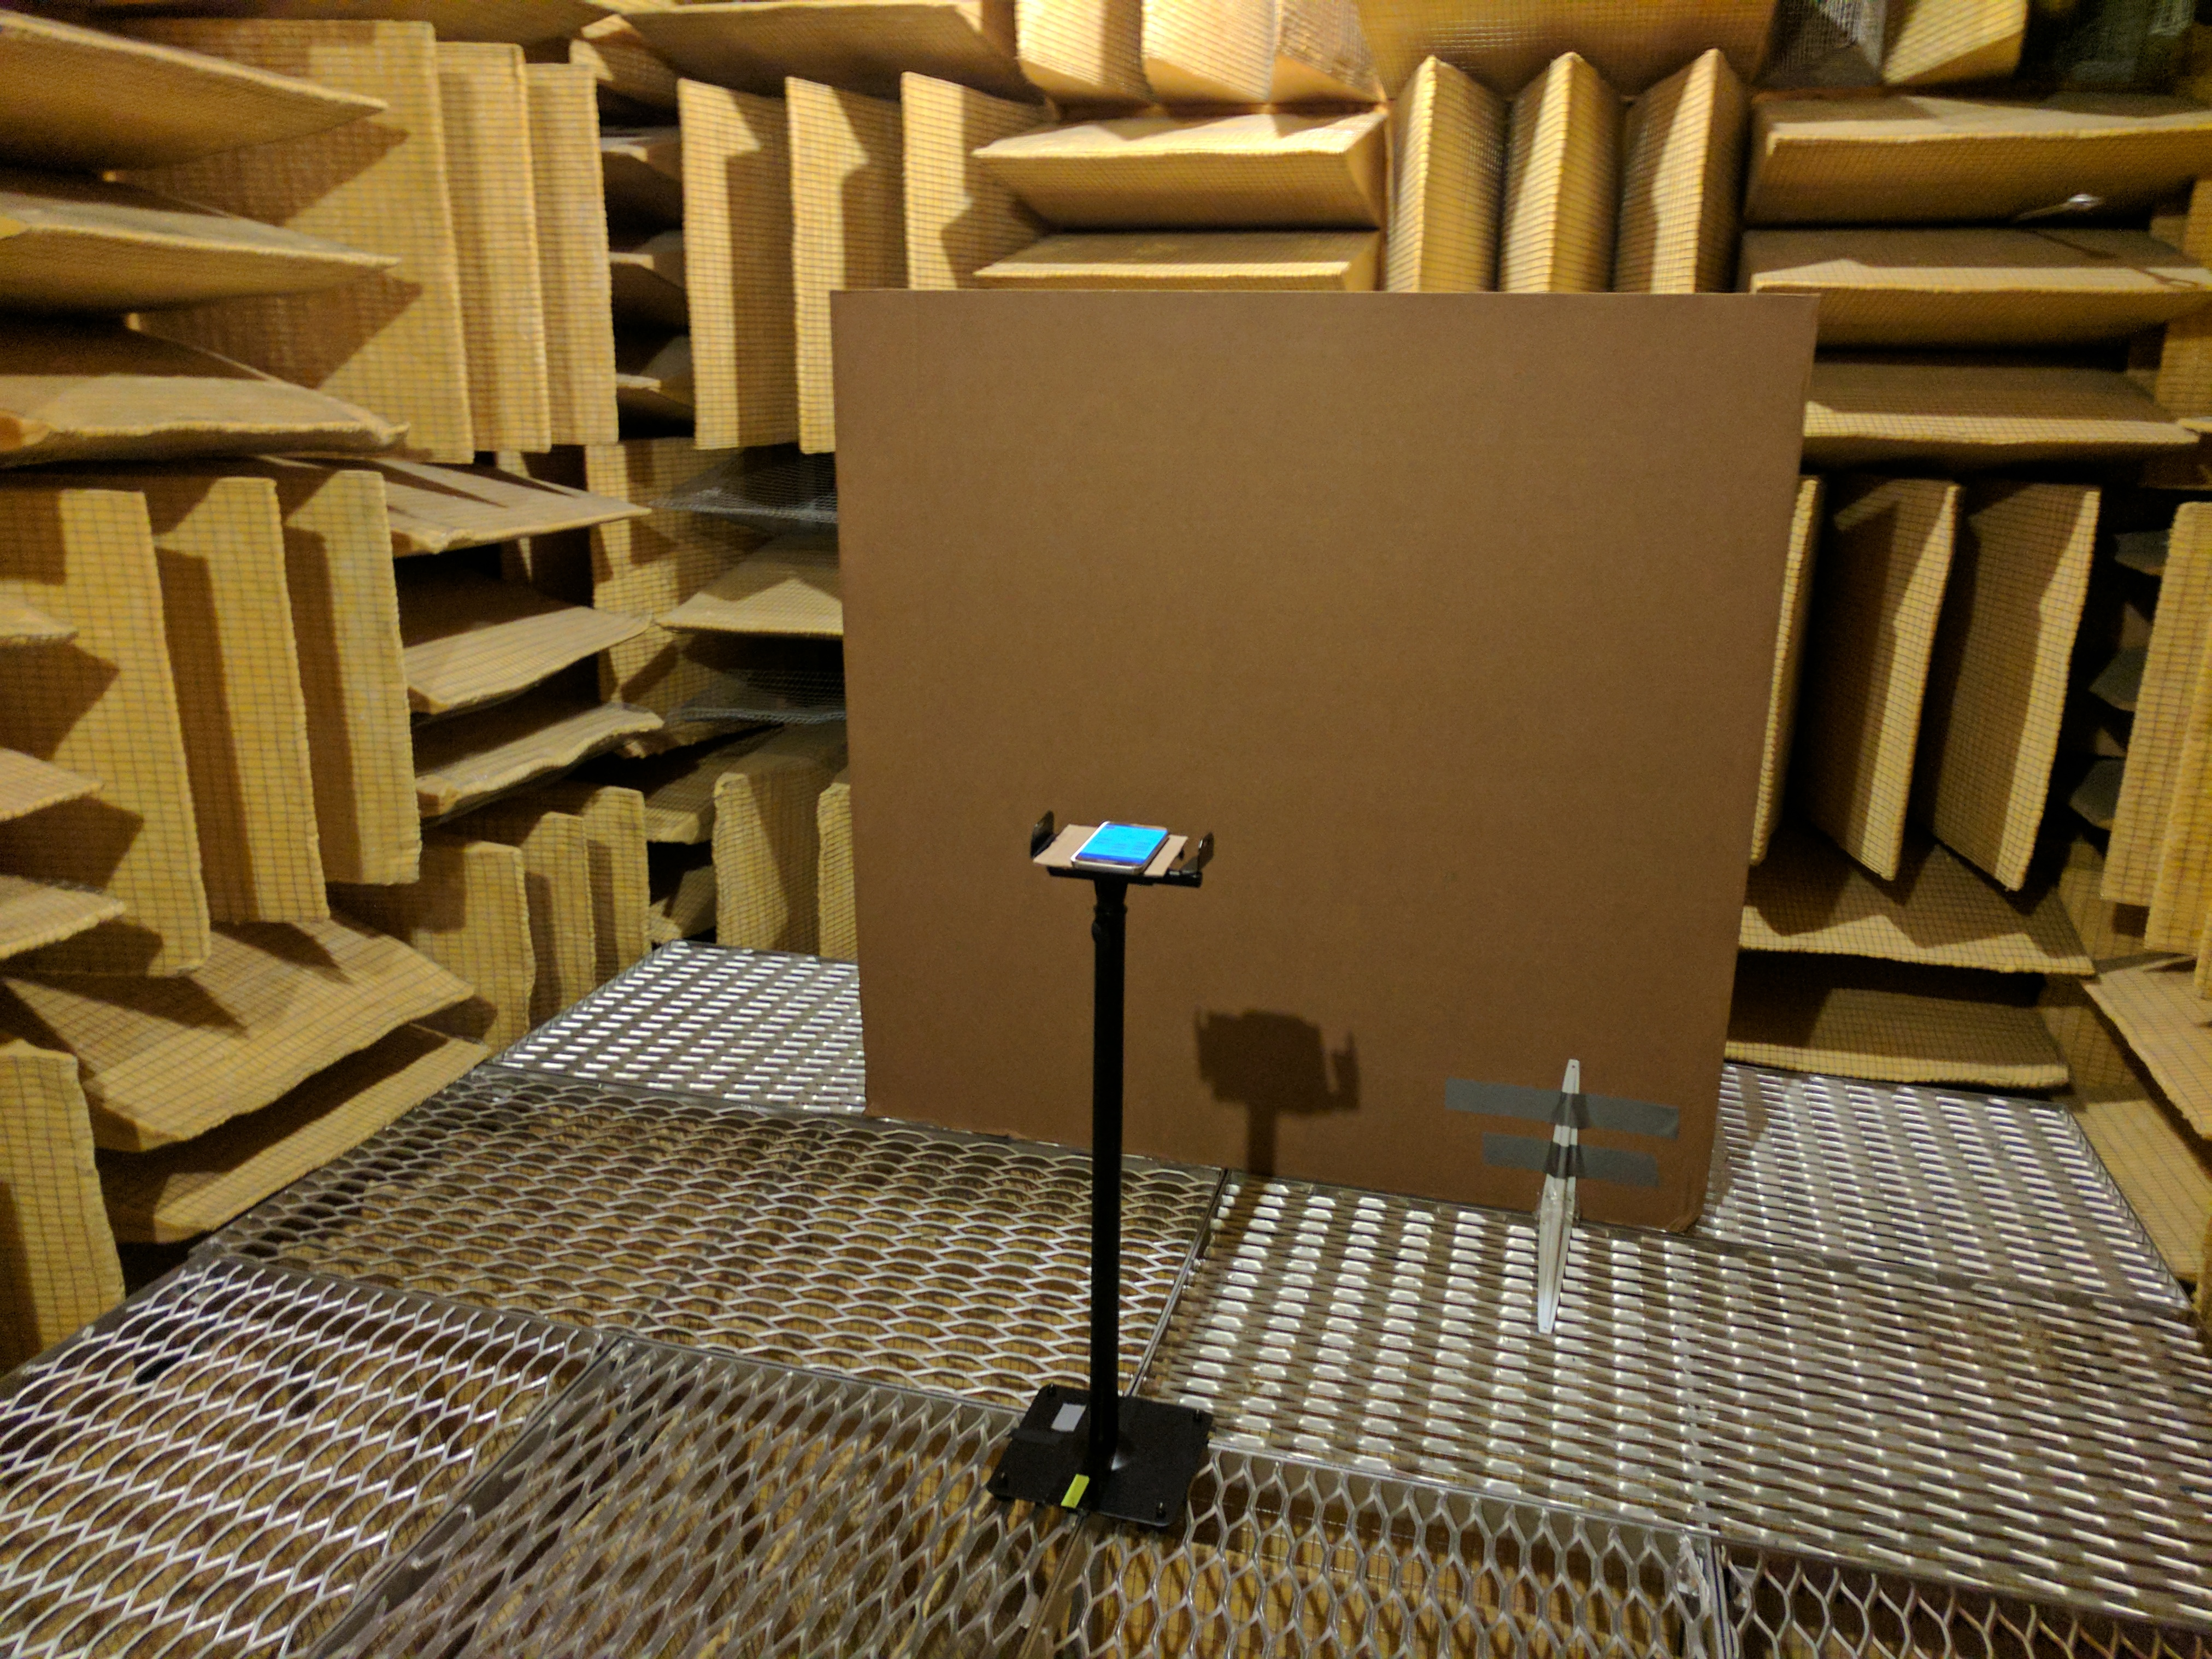
\includegraphics[width=0.40\columnwidth, %keepaspectratio]{figs/anechoic_experiment.jpg}}
%    \label{fig:anechoic}
%}

\section{\emph{Batphone} : System Overview}\label{sec:overview}

Fig.~\ref{fig:batphone_vision} illustrates how the system will work.
\begin{figure}[h!t]
%\vspace{-0.1in}
\center{
\includegraphics[width=\columnwidth]{figs/Batphone.pdf}
%\vspace{-0.1in}
\caption{{\small Batphone}}
%\vspace{-0.1in}
\label{fig:batphone_vision}
}
\end{figure}

Following are the building blocks coupled with their description :
\subsubsection{Dead Reckoning}
\begin{itemize}
\item Step size estimation
\item Step detection and count
\item Heading direction
\item Phone orientation
\end{itemize}

\subsubsection{FMCW based distance}
\begin{itemize}
\item FMCW parameter choices ( Chirp duration, Mic choice, Frequency response of speaker and mic based selection, Gap between chirps, Bandwidth selection, Sampling rate selection (Higher means lower quantization error or can also be done with zero padding). )
\item Synchronization with dead reckoning.
\item FMCW profile based corner detection and clutter filtering.
\end{itemize}

\subsubsection{Room shape profiling}
\begin{itemize}
\item Geometric constraints on the room wall and movement.
\item Corner detection help in profiling.
\end{itemize}
\section{Design choices}
\label{sec:design}

\subsection{Different False Attempts or Starts}
\begin{itemize}
\item Pulse based echo selection and finding or Echo-sorting (Too much direct path impact).
\item Angle-of-arrival calculation (Too less number of mics and sine based or CIR based phase measurement won't work due to high level of multi-path).
\item MUSIC based peak selection (Prior knowledge of number of peaks).
\end{itemize}

\subsection{FMCW based observations}

\subsubsection{Resolution}
It depends upon the bandwidth used.

\begin{figure}[hbt]

\centering{
\subfigure[4KHz]{
    \includegraphics[width=0.46\columnwidth, keepaspectratio]{figs/4K.pdf}
    \label{fig:4K}
}
\subfigure[10 KHz ]{

    \includegraphics[width=0.46\columnwidth,  keepaspectratio]{figs/10K.pdf}
    \label{fig:10K}

}
%\vspace{-0.15in}
\caption{Impact of different bandwidths on resolution FMCW based distance measurement}
%\vspace{-0.15in}
\label{fig:resolution}
}
\end{figure}

\subsubsection{Volume Level}
It depends upon the proper volume level used.


\begin{figure}[hbt]

\centering{
\subfigure[Amplitude]{
    \includegraphics[width=0.46\columnwidth, keepaspectratio]{figs/volume-amp.pdf}
    \label{fig:amp}
}
\subfigure[SNR]{

    \includegraphics[width=0.46\columnwidth,  keepaspectratio]{figs/volume-snr.pdf}
    \label{fig:snr}

}
%\vspace{-0.15in}
\caption{{Impact of different volume level on FMCW based distance measurement}
%\vspace{-0.15in}
\label{fig:volume}
}
}
\end{figure}

\subsubsection{FMCW distance measurement with sizes}
It depends upon the reflection measurement with sizes.

\begin{figure}[h!t]
%\vspace{-0.1in}
\center{
\includegraphics[width=\columnwidth]{figs/distance_error.pdf}
%\vspace{-0.1in}
\caption{FMCW error change with distance}
%\vspace{-0.1in}
\label{fig:distance_error}
}
\end{figure}

\begin{figure}[h!t]
%\vspace{-0.1in}
\center{
\includegraphics[width=\columnwidth]{figs/size_error.pdf}
%\vspace{-0.1in}
\caption{FMCW amplitude with different sizes}
%\vspace{-0.1in}
\label{fig:size_error}
}
\end{figure}

\begin{figure}[h!t]
%\vspace{-0.1in}
\center{
\includegraphics[width=\columnwidth]{figs/cdf-localization.pdf}
%\vspace{-0.1in}
\caption{{\small CDF of FMCW based distance calculation error.}}
%\vspace{-0.1in}
\label{fig:cdf}
}
\end{figure}
\begin{figure}[h!t]
%\vspace{-0.1in}
\center{
\includegraphics[width=\columnwidth]{figs/angle.pdf}
%\vspace{-0.1in}
\caption{{\small Perpendicular distance measured at different angles.}}
%\vspace{-0.1in}
\label{fig:angle}
}
\end{figure}
\begin{itemize}
\item Junction causes mutliple peaks.
\item Maximum peak in FMCW corresponds to the main wall distance.
\item Always get perpendicular distance from wall.
\item Peak amplitude increases with the size of the reflector and it saturates after certain size.
\item Corner peaks are significantly different (at least for corner less than or equal to 90 degree). There are multiple peaks and peak spread is more.
\item Audio lobe direction and mic position matters.
\end{itemize}

\section{Algorithm Description}\label{sec:algo}

Description of the algorithm and geometric arguments with some explanatory figures. Fig.~\ref{fig:roomshape_algo} illustrates the algorithm used in room shape detection.

\begin{figure}[h!t]
\center{
\fbox{\includegraphics[width=\columnwidth]{figs/roomshape_algo.pdf}}
\caption{Algorithm sketch of \textit{Batphone}}
\label{fig:roomshape_algo}
}
\end{figure}

\begin{algorithm}
    %\vspace{-12pt}
    \caption{\singletag}\label{alg:batphone}
    \begin{algorithmic}[1] 
        \State $x_0 \gets $ current phone orientation 
        \State $p(x) \gets $ current position of the person

        \Procedure{Step Detection}{$\mathbf{a}$}
         		\If{$Acc > Th$}
                    \textbf{return} \texttt{True}
                \EndIf
            \State \textbf{return} \texttt{False}
        \EndProcedure

        \Procedure{getDeadReckoning}{}
            \State $t_0 \gets $ \textsc{currentSystemTime} 
            \State $t \gets t_0$
            \State $\mathbf{w} \gets $ \textsc{emptyVector}
%            \While{$t \leq t_0 + T$}
%                \State $t \gets $ \textsc{currentSystemTime}
%                \State $\mathbf{w} \gets $ \textsc{append}($\mathbf{w}$,
%                    \textsc{currentPhaseReading})
%            \EndWhile
            \State \textbf{return} \texttt{True}
        \EndProcedure

        \Procedure{updateLocation}{$x_0, \mathbf{w}$}
            \State $x_\mathrm{new} \gets \argmin_{x_\mathrm{min} < x <
                x_\mathrm{max}} $ \Call{minDTW}{$x_0, x, \mathbf{w}$}
            \State \textbf{return} $x_\mathrm{new}$
        \EndProcedure

%        \Procedure{touchDetection}{}
%            \While{\texttt{True}}
%                \State $\mathbf{w} \gets $\Call{getPhaseData}{} 
%                \If{$\mathbf{mean}(\mathbf{w}) > C$}
%                    \textbf{return} \texttt{True}
%                \EndIf
%            \EndWhile
%        \EndProcedure
%
%        \Procedure{touchTracking}{}
%            \While{\texttt{True}} 
%                \State $\mathbf{w} \gets $\Call{getPhaseData}{} 
%                \State $x_0 \gets $ \Call{updateLocation}{$x_0, \mathbf{w}$}
%            \EndWhile
%        \EndProcedure
%
%        \State \textsc{touchDetection}();
%        \State \textsc{touchTracking}();
    \end{algorithmic}
    %\vspace{-12pt}
\end{algorithm}
\section{Geometric Constraints}\label{sec:geometric}
Once we have synchronized position samples ($x_t,y_t$) from dead-reckoninig and range readings ($r_t$) from FMCW, we now need to estimate the coordinates of the points on the wall that we received reflection ($(x'_t,y'_t)$) from and those points we estimate the wall.
Since the range values are prependicular distances from the wall we get the following two geometric constraints on the values of $(x_t',y_t')$.
$$(y_t' - y_t)^2 + (x_t' - x_t)^2 = r_t^2$$.
$$\frac{y_t' - y_t}{x_t' - x_t} = \frac{-1}{m_2}$$ 

Where $m_2$ is the gradient of wall. To calculate $m_2$ we get the wall orientation with respect to the path traversed by the phone, as shown in fig XXX,  is given as $\theta = sin^{-1}(\frac{d_t}{\textbf{X}})$. Using similar triangle property $\textbf{X} = \frac{d_t \sqrt{(y_{t+1} - y_t)^2 + (x_{t+1} - x_t)^2}}{d_{t+1} - d_t}$, thus giving us 
$$\theta = sin^{-1}(\frac{d_{t+1}-d_t}{\sqrt{(y_{t+1} - y_t)^2 + (x_{t+1} - x_t)^2}})$$.

$m_2$ can now be calculated as $m_2 = tan(\theta + tan^{-1}(m_1))$, or $m_2 = tan(-\theta + tan^{-1}(m_1))$ depending on the side of the path the reflecting wall is present. Here $m_1 = \frac{y_{t+1} - y_t}{x_{t+1} - x_t}$ is the gradient of the path traversed.

Using these constraints $x_t'$ and $y_t'$ can be calculated as
$$x_t' = \pm \sqrt{r_t^2 * \frac{m_2^2}{m_2^2+1}} + x_t; $$
$$y_t' = (x_t-x_t')/m_2 + y_t$$

This would give us four set of values for $x_t'$ and $y_t'$, two on each side of the path. Using the phone orientation we know which side of the path the wall is enabling us to filter out two set of values. Among the remaining two we pick the set of values which would satisfy the following simple constraint
$$\frac{y_{t+1}' - y_t'}{x_{t+1}' - x_t'} = m_2$$
%\begin{figure}[hbt]
%  %\vspace{-0.15in}
%\centering{
%\subfigure[]{
%    \fbox{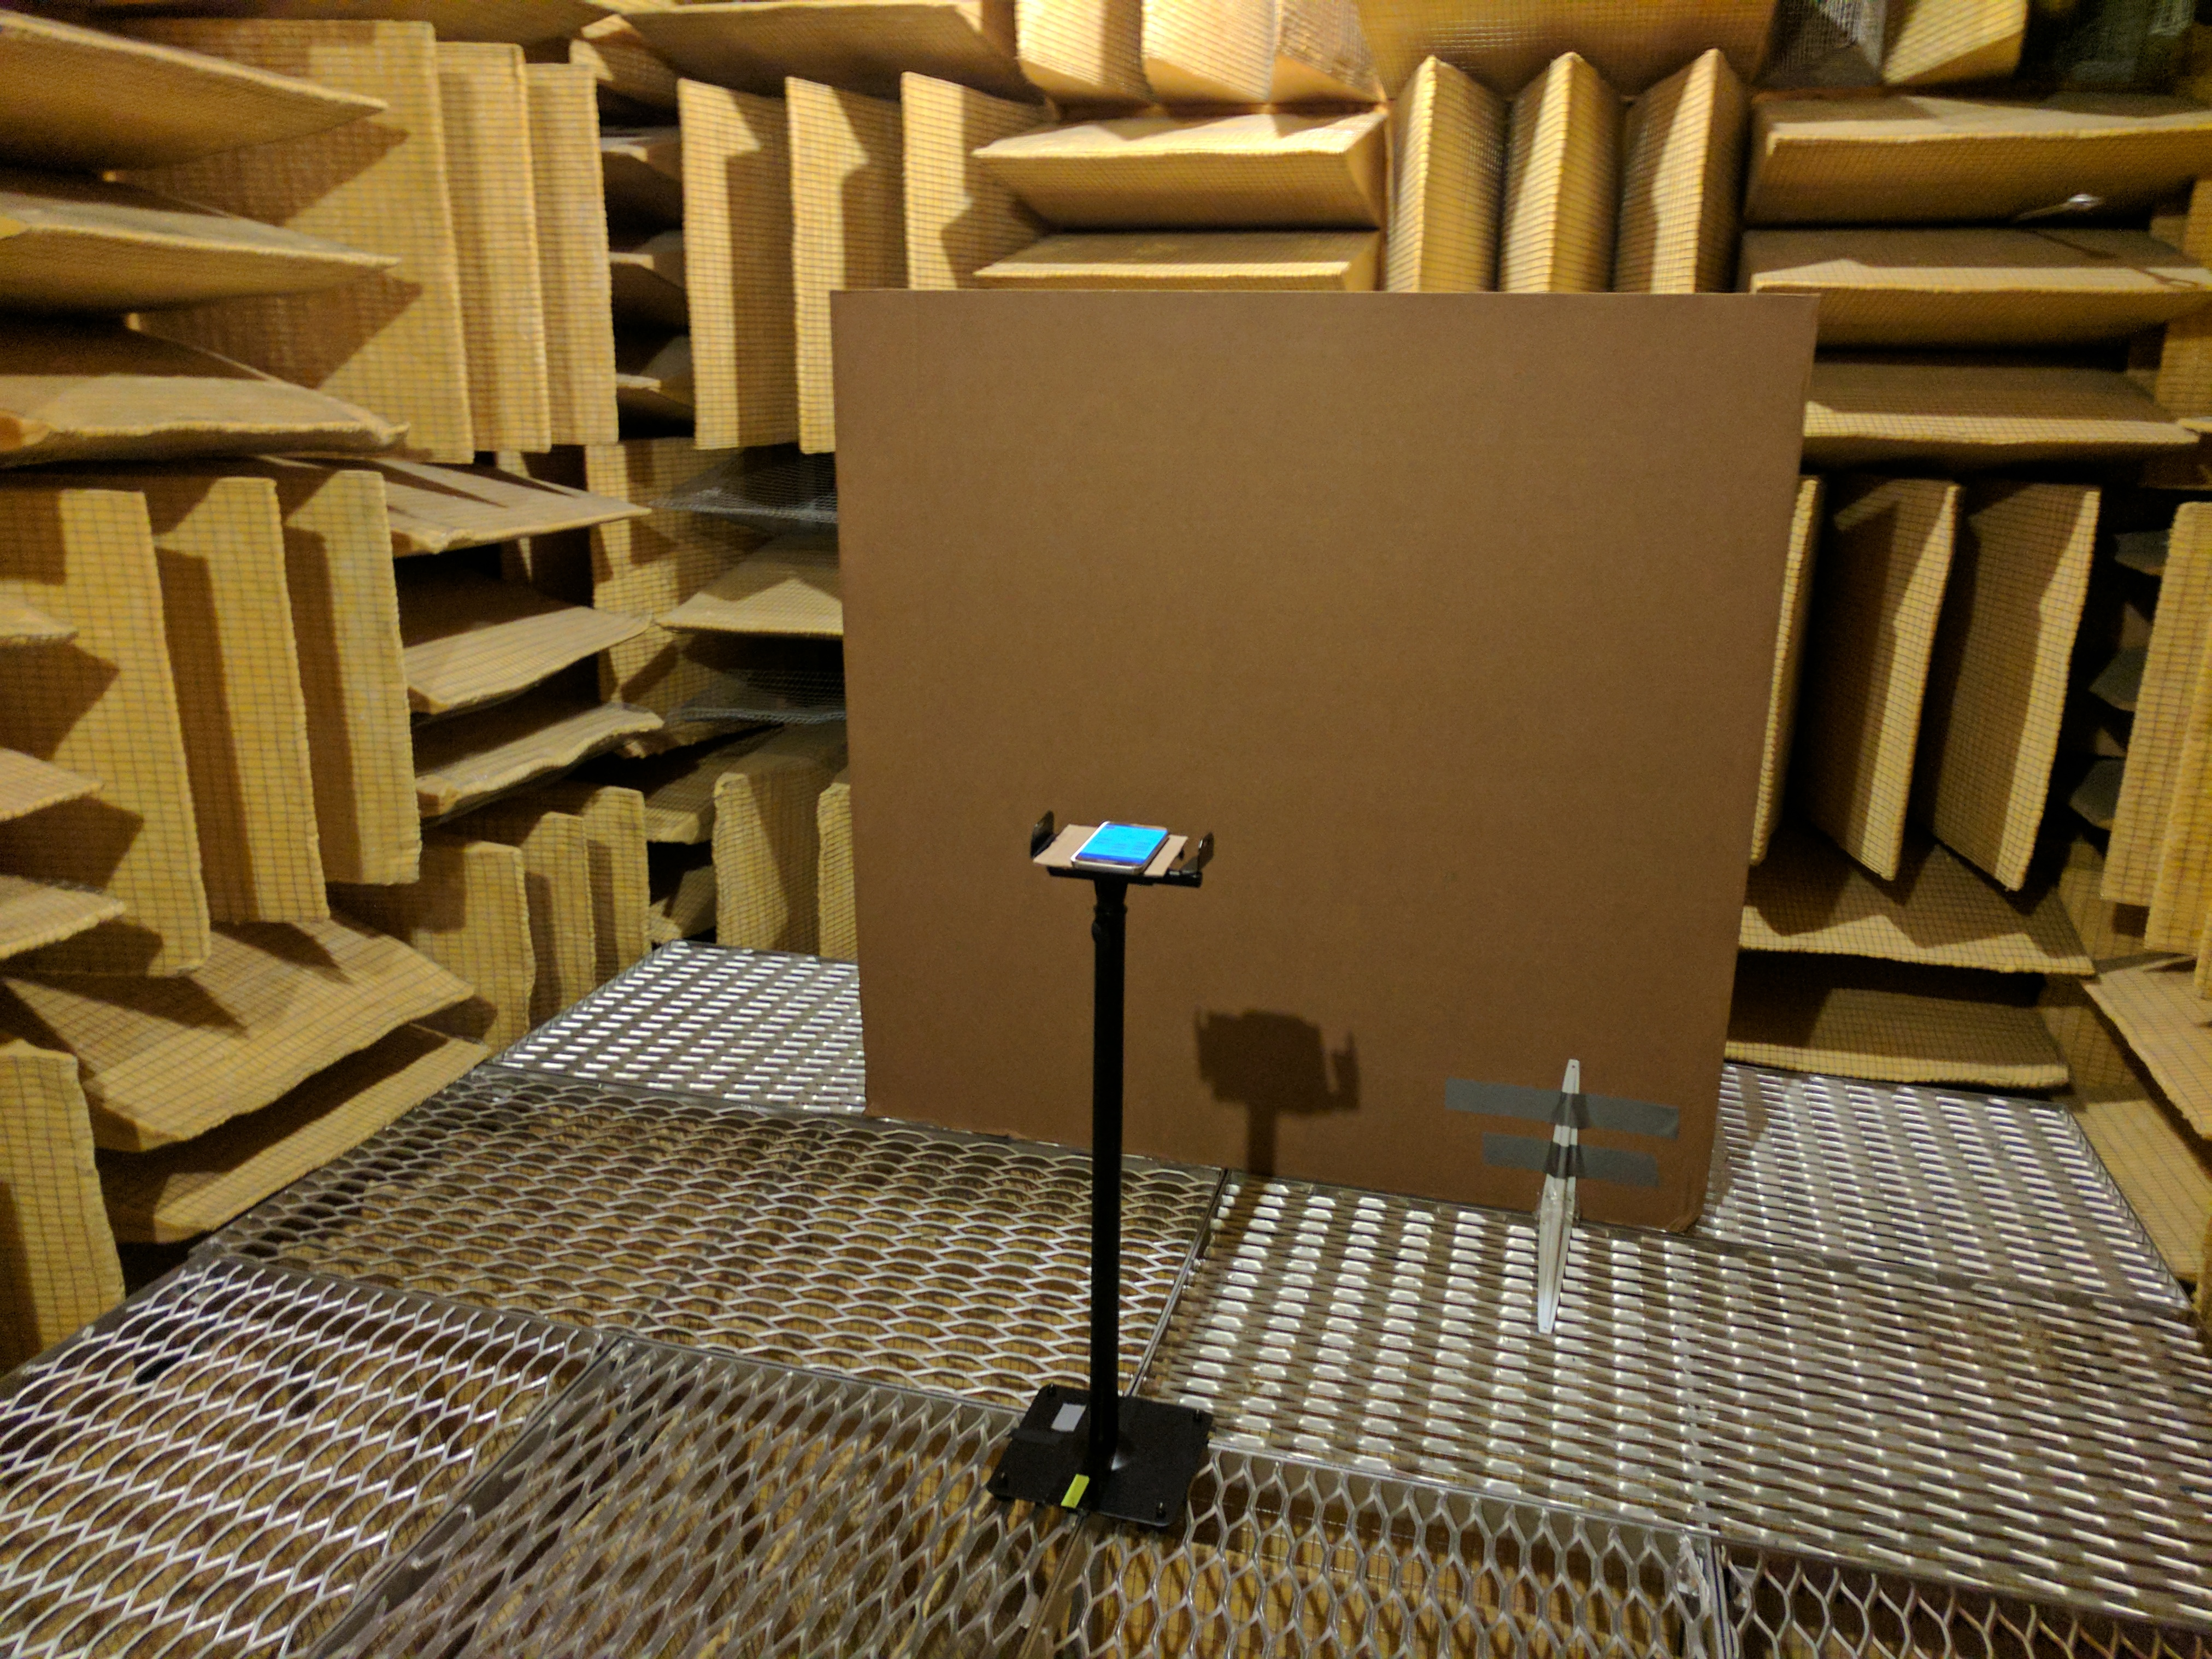
\includegraphics[width=0.40\columnwidth, %keepaspectratio]{figs/anechoic_experiment.jpg}}
%    \label{fig:anechoic}
%}

\section{Setup}\label{sec:setup}
In this section, we describe our different experimental setups in detail. 

\begin{figure}[h!t]
\center{
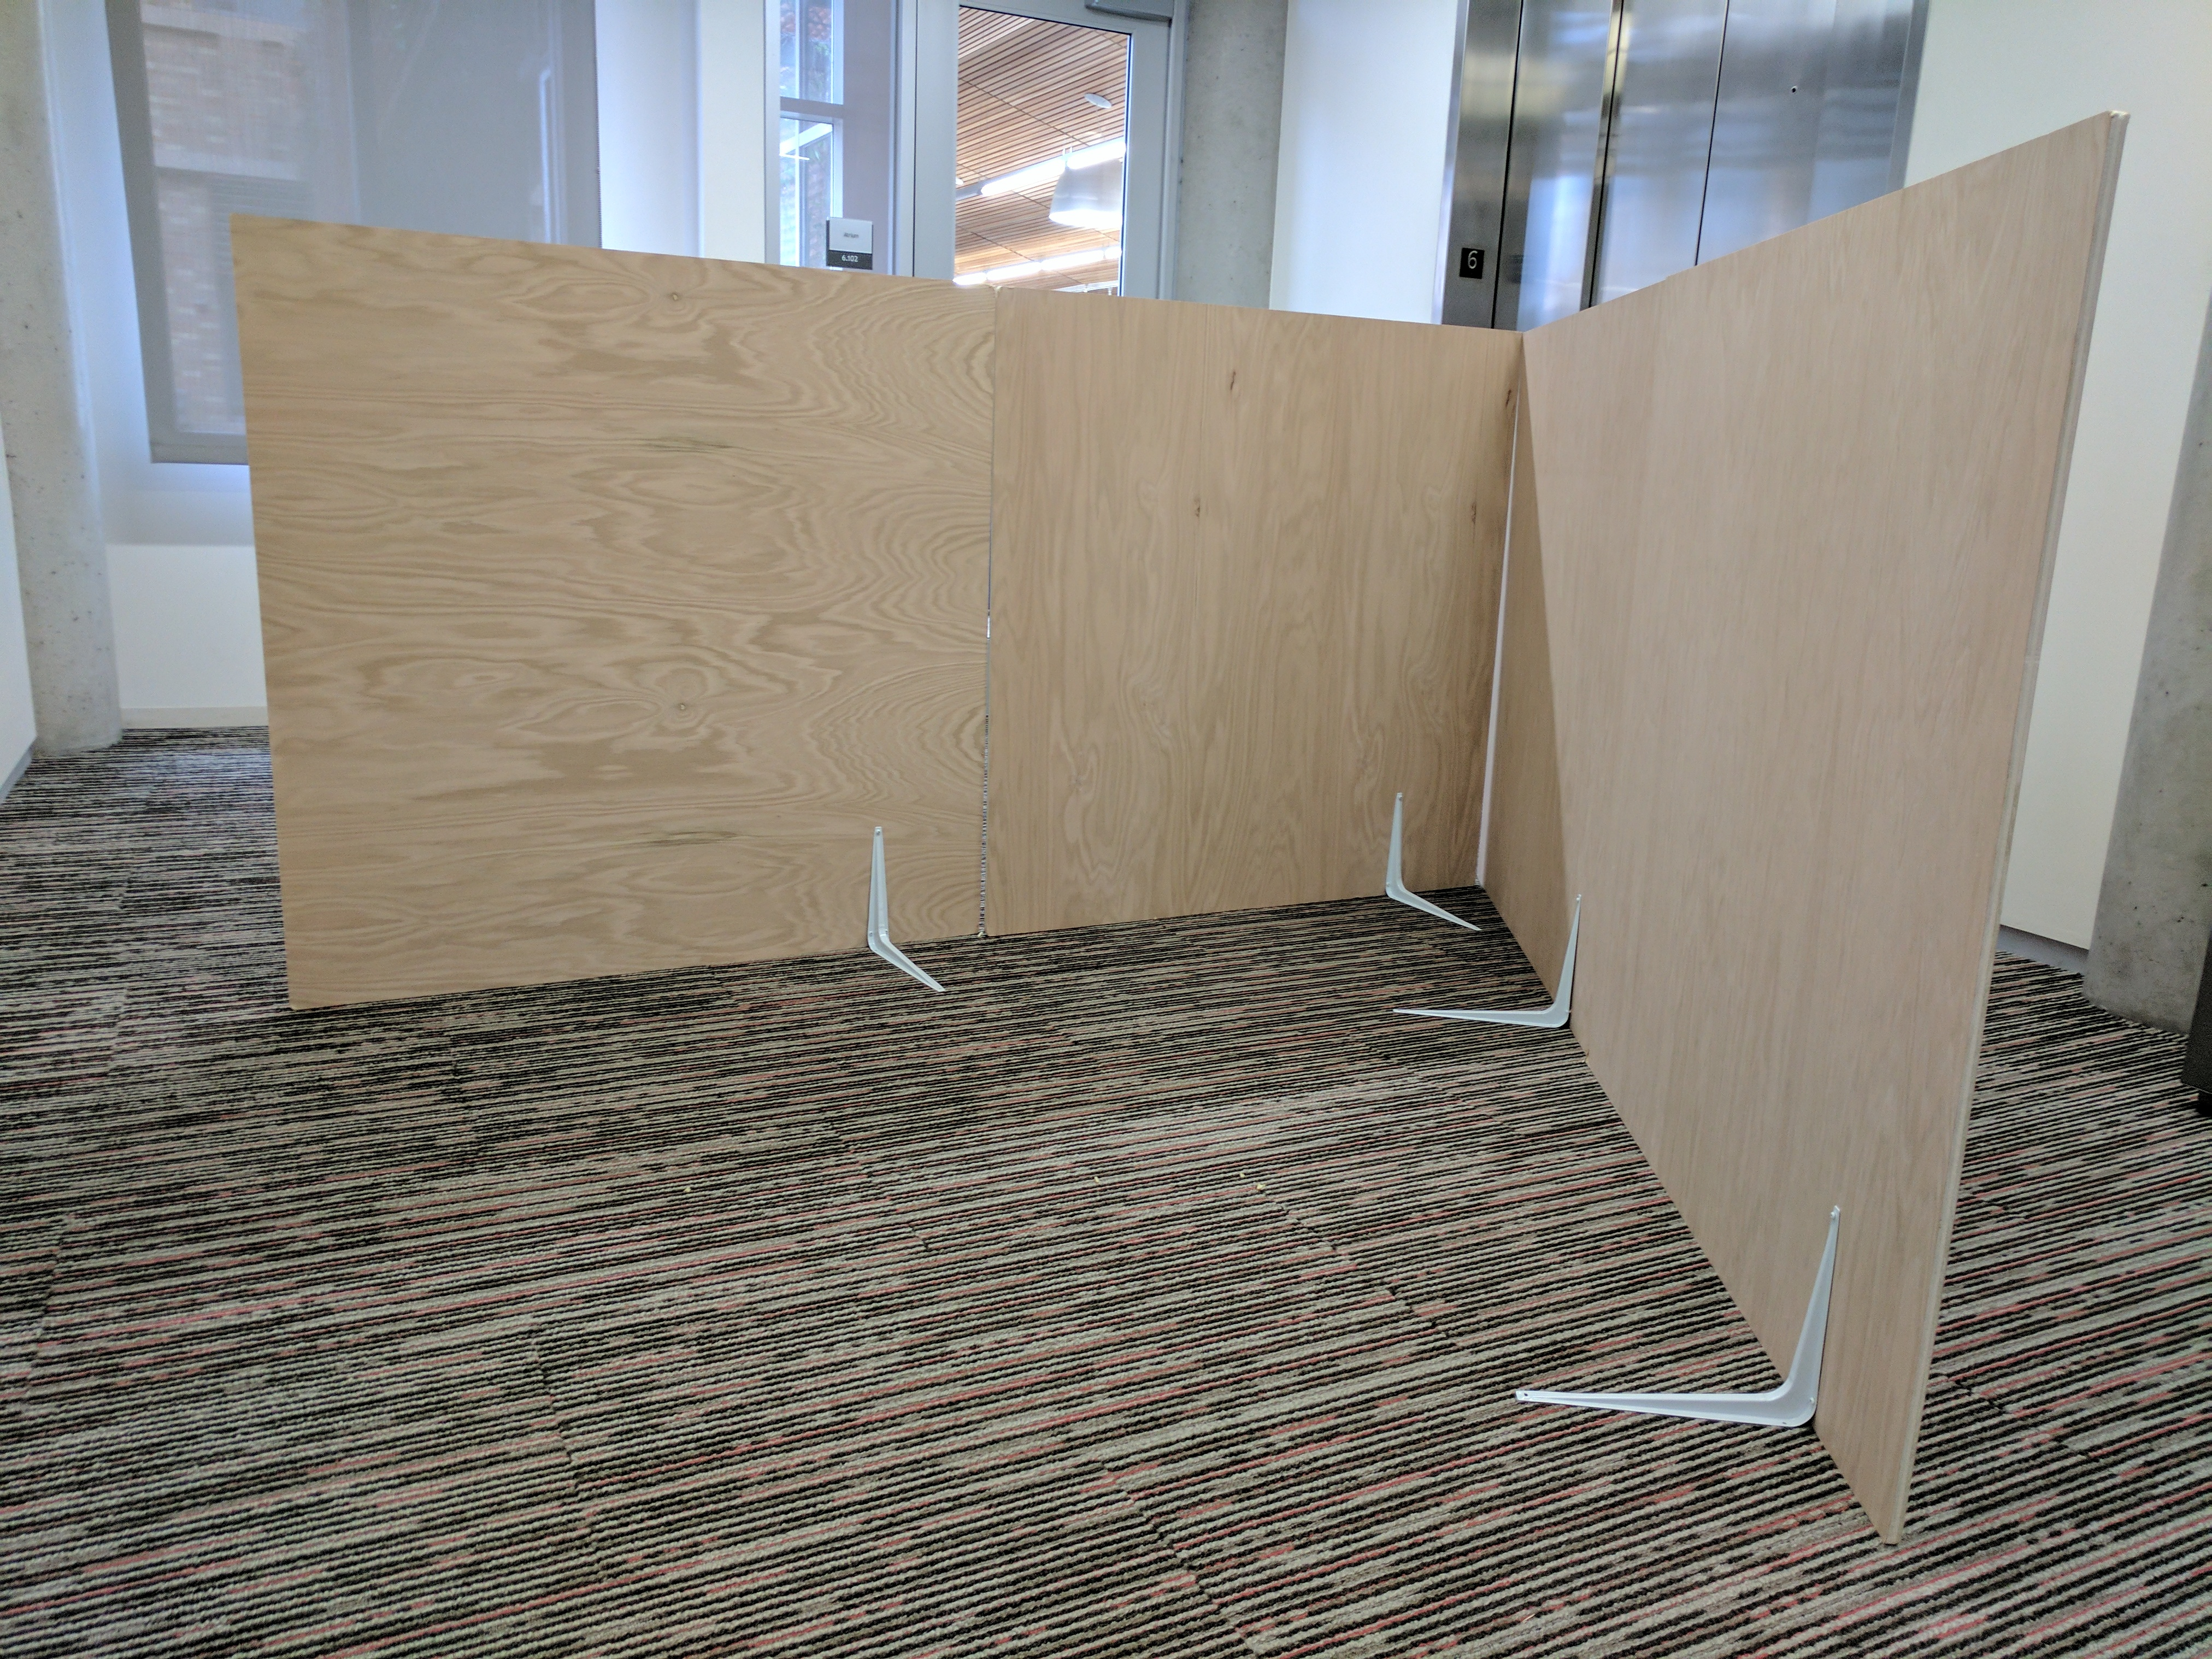
\includegraphics[width=\columnwidth]{figs/contour_experiment.jpg}
\caption{Contour Experiment}
\label{fig:contour}
}
\end{figure}

\begin{figure}[hbt]
  %\vspace{-0.15in}
\centering{
\subfigure[]{
    \fbox{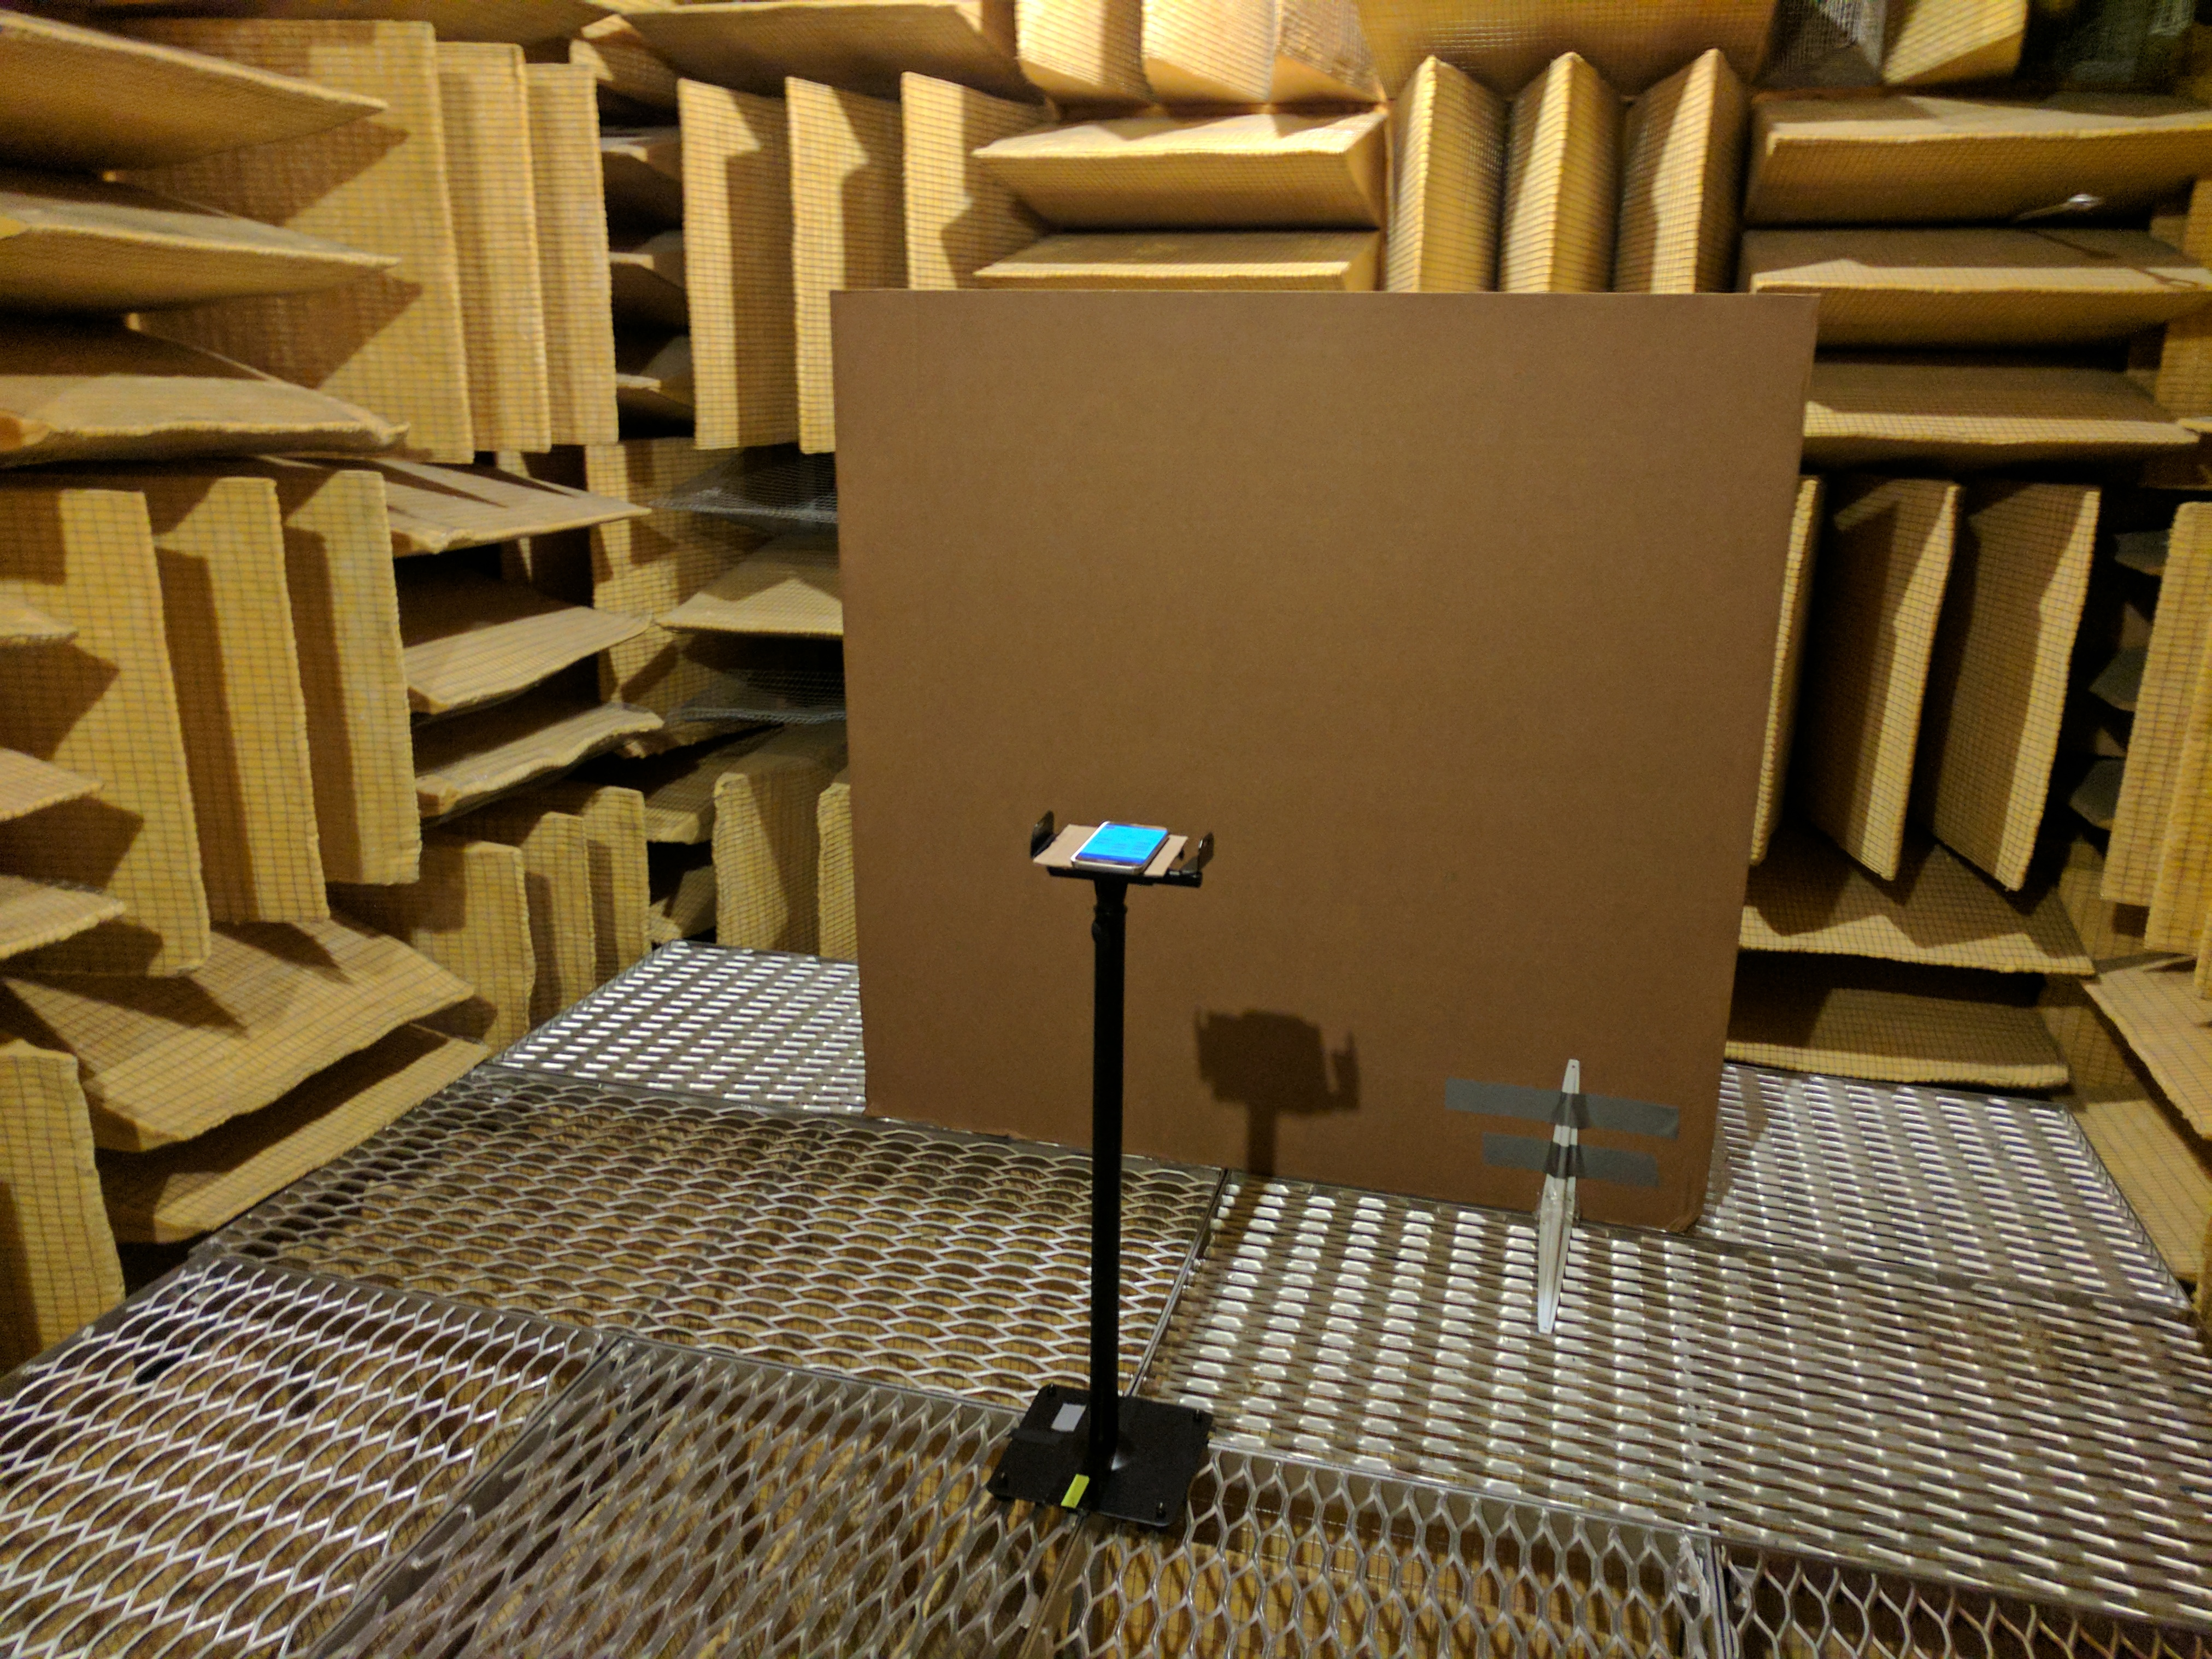
\includegraphics[width=0.40\columnwidth, keepaspectratio]{figs/anechoic_experiment.jpg}}
    \label{fig:anechoic}
}
\subfigure[]{

    \fbox{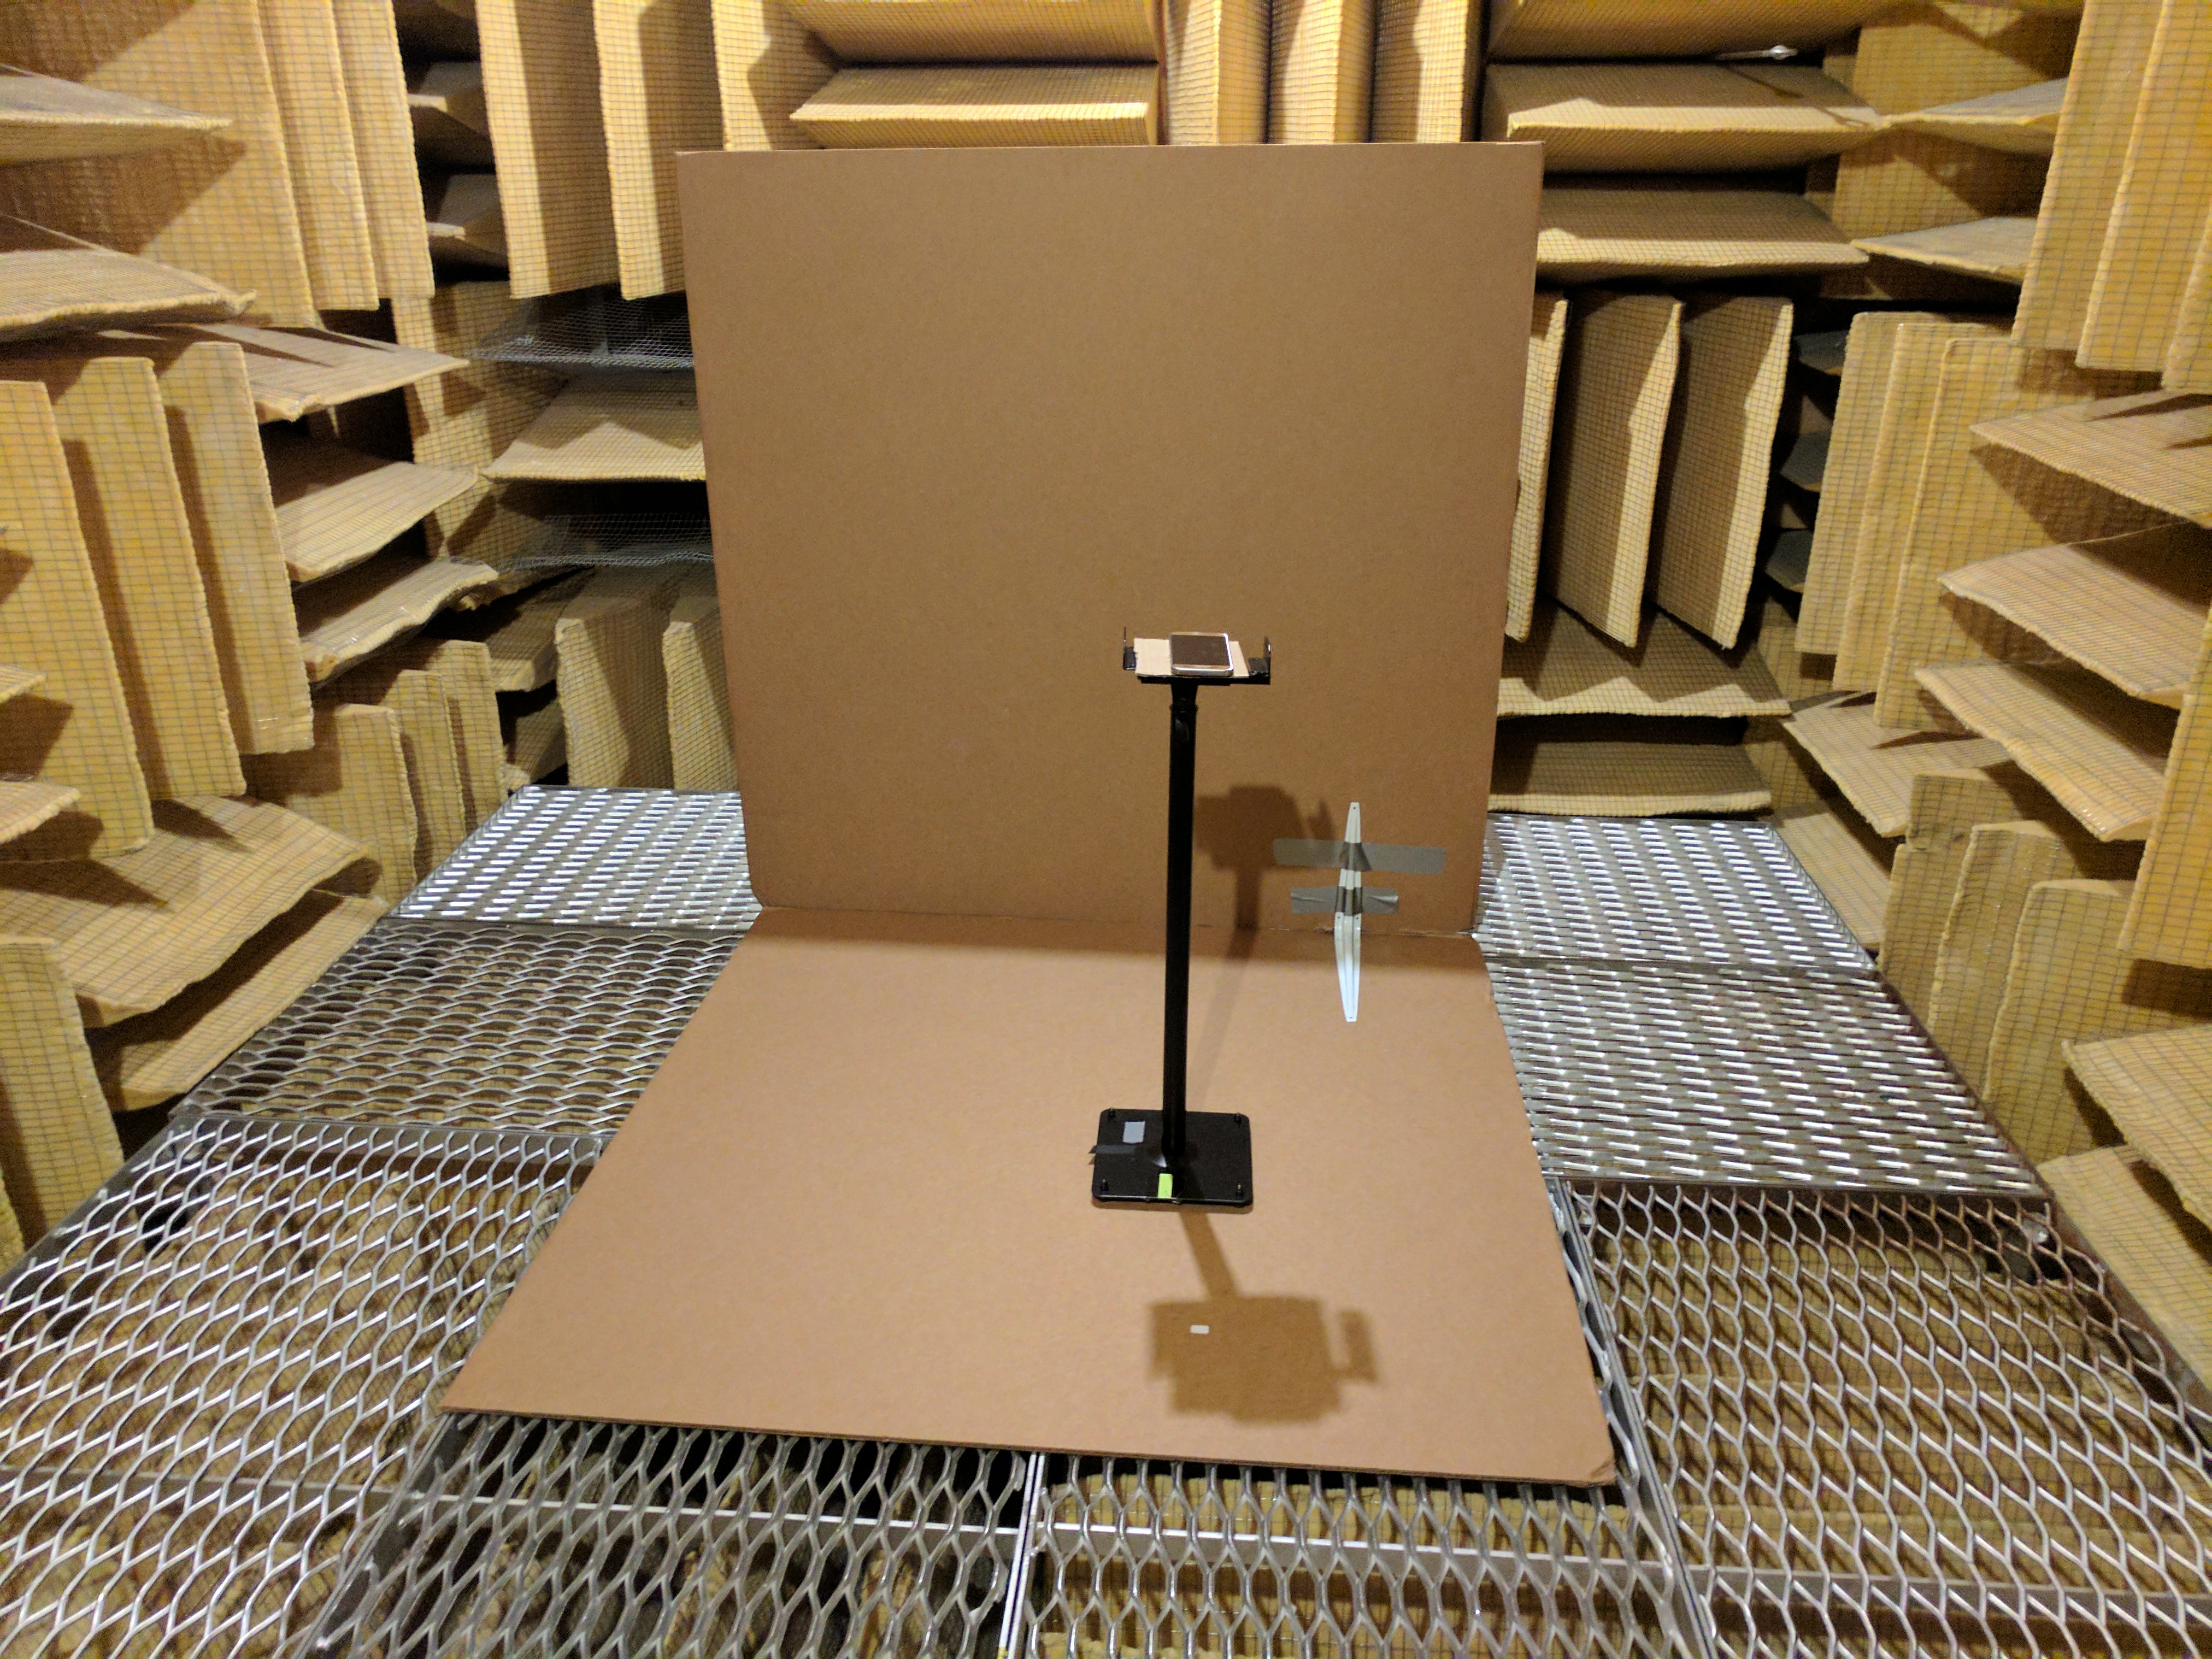
\includegraphics[width=0.40\columnwidth,  keepaspectratio]{figs/anechoic_experiment_floor.jpg}}
    \label{fig:anechoic_floor}

}
%\vspace{-0.15in}
\caption{{\small (a). Anechoic Experiment 1. (b).  Anechoic Experiment 2. }}
%\vspace{-0.15in}
\label{fig:anechoic}
}
\end{figure}


\input{metrics}
\section{Evaluation}\label{sec:results}
This is result section.

\subsection{Micro-benchmark for FMCW}

    - Different distance measurement accuracy

    - Wall orientation w.r.t path of the phone accuracy (Showing one gets perpendicular distance)
 
    - Resolution of distance measurement accuracy

    - Reflector size

   - Impact of phone height (peaks from ceiling + floor) and phone holding pattern
   
\subsection{Dead-reckoning based estimation}
   - Path profiling error (accelerometer + gyro)
   \begin{figure}[h!t]
   \center{
   \includegraphics[width=\columnwidth]{figs/cdf-localization-deadreckoning.pdf}
   \caption{Dead-reckoning based distance estimation error.}
   \label{fig:with_dead_reckoning}
   }
   \end{figure}
   
\subsection{Single wall Contour}

  - Different shape Straight and Angled
 
   - Also need to try more shapes and sizes

\subsection{Multi wall Contour}

  Corner detection accuracy (False positive rate)
  
  Closed Intersections
   
  - Different angles
 
  - Different sized walls in intersection
  
  - Direction association accuracy (If you are moving along a straight line and you have one wall in right or left side. How do you know which side is your wall ?)
  
  Semi-Closed intersections
  
\begin{figure}[h!t]
\center{
\includegraphics[width=\columnwidth]{figs/anechoic/8by8.jpg}
\caption{FMCW based and peak detection for distance measurement}
\label{fig:fmcw_distance}
}
\end{figure}

\begin{figure}[h!t]
\center{
\includegraphics[width=\columnwidth]{figs/anechoic/with_floor_60_s2.jpg}
\caption{With floor}
\label{fig:with_floor}
}
\end{figure}

\begin{figure}[h!t]
\center{
\includegraphics[width=\columnwidth]{figs/anechoic/without_floor_60.jpg}
\caption{Without floor}
\label{fig:without_floor}
}
\end{figure}

\subsection{Multi wall Contour with clutter}

Sensitivity to surrounding small objects by trying to add different sizes small objects at different locations to see if you can effectively filter them out 
%\section{\emph{Batphone} : System Overview}\label{sec:overview}

Fig.~\ref{fig:batphone_vision} illustrates how the system will work.
\begin{figure}[h!t]
%\vspace{-0.1in}
\center{
\includegraphics[width=\columnwidth]{figs/Batphone.pdf}
%\vspace{-0.1in}
\caption{{\small Batphone}}
%\vspace{-0.1in}
\label{fig:batphone_vision}
}
\end{figure}

Following are the building blocks coupled with their description :
\subsubsection{Dead Reckoning}
\begin{itemize}
\item Step size estimation
\item Step detection and count
\item Heading direction
\item Phone orientation
\end{itemize}

\subsubsection{FMCW based distance}
\begin{itemize}
\item FMCW parameter choices ( Chirp duration, Mic choice, Frequency response of speaker and mic based selection, Gap between chirps, Bandwidth selection, Sampling rate selection (Higher means lower quantization error or can also be done with zero padding). )
\item Synchronization with dead reckoning.
\item FMCW profile based corner detection and clutter filtering.
\end{itemize}

\subsubsection{Room shape profiling}
\begin{itemize}
\item Geometric constraints on the room wall and movement.
\item Corner detection help in profiling.
\end{itemize}
\section{Points of Discussion}
Following are the points we learned.

\section{Related Work}\label{sec:related}
Acoustic echoes reveal room shape \cite{ranking_echoes,room_shape,echo_slam,bat_echo}

Finding source of audio \cite{audio_source}.
Acoustic signals improve $3D$ visualization \cite{geom_echo}.

Sound-based smartphone proximity detection \cite{sound_prox}. Sound based encounter detection \cite{dopenc}. Ambient sound finger-printing based room detection \cite{batphone_abs}. Sound-reflection signature based position detection \cite{echotag}. 

Software sonar sensor \cite{iot15}, Floor-plan with ultra-sonic sensor \cite{ccnc16},

Tracking ( FingerIO \cite{fingerio}, CAT \cite{cat}, aamouse \cite{aamouse}  \cite{audiogest}).

Ambinet sound based fingerprinting. \cite{soundsense, surroundsense} and sound based indoor localization \cite{soundloc, roomsense}.

Infrastructure-based acoustic indoor localization system \cite{assist, iphone_soundloc,beep,beepbeep,indoor_ambient,walrus}.

Smartphone-based $2D$-mapping \cite{iot15, iot16}.

Audio based phone range-finder \cite{phone_lidar}.




%\section{Future works}
This is future works.

\section{Conclusion}
\label{sec:conclusion}
This is Conclusion.


%\bibliographystyle{splncs03}
\bibliographystyle{ieeetr}
\bibliography{main}
%\small\bibliography{main}
\end{document}
